\begin{figure*}[t]
    \centering
    
\includegraphics[width=\linewidth]{figures/pipeline.pdf}
\caption{
\textbf{Overview of the \methodname{} pipeline.}
Given an input mesh, \methodname{} casts UV seam cutting as generation on the mesh graph.
We build a mesh graph with geometric and topological features and parameterize the flow model with a Mesh Transformer.
Each block first applies global self-attention to position-aware vertex features, and then uses edge-featured graph attention to propagate local connectivity cues and update both vertex and edge features in a topology-aware manner.
Starting from random edge noise, the model generates a coherent per-edge seam mask, which is converted into seam cuts and used to unwrap the mesh into a UV atlas.
}
    \label{fig:pipeline}
\end{figure*}

\section{Method}
% Overview of the SeamGen pipeline. Our method frames UV seam generation as a distribution modeling problem on mesh graphs. Given an input mesh, we first construct a mesh graph incorporating geometric and topological edge features. A mesh-native transformer is then used to parameterize a flow-matching model. The model generates a coherent per-edge seam field, initialized from random edge noise, which is subsequently converted into seam cuts and used to unwrap the mesh into a UV atlas.

% Our method formulates UV seam generation as learning the distribution of artist-authored seam layouts directly on the mesh graph. To this end, we instantiate a flow matching model for seam generation (see Sec.~\ref{sec:formulation}), parameterize it with a Mesh Transformer that captures both global and local mesh cues (see Sec.~\ref{sec:backbone}), and further exploit training-free inpainting for progressive refinement of problematic samples (see Sec.~\ref{sec:inpainting}). The overall pipeline is illustrated in Fig.~\ref{fig:pipeline}.

Given an input mesh, our method generates a per-edge seam layout, represented as a binary seam mask over mesh edges, which is then used to unwrap the mesh into a UV atlas.
% We formulate this task as learning the distribution of artist-authored seam layouts directly on the mesh graph.
We formulate this task as conditional seam generation on the mesh graph, where the model learns to capture the distribution of artist-authored seam layouts conditioned on the input mesh.
To this end, we instantiate a flow matching model for seam generation (Sec.~\ref{sec:formulation}), parameterize it with a Mesh Transformer that captures both global and local mesh cues (Sec.~\ref{sec:backbone}), and exploit the learned flow model as a training-free conditional generative prior, supporting both constraint-guided seam completion from sparse user inputs and automatic self-refinement of problematic UV regions (Sec.~\ref{sec:inpainting}). The overall pipeline is illustrated in Fig.~\ref{fig:pipeline}.



\subsection{Seam Cutting as Generation}
\label{sec:formulation}
% A high-quality UV seam layout is rarely determined by a small set of explicit objectives. 
% Artist-authored seams encode a mixture of geometric, perceptual, semantic, and practical preferences: they are often placed along sharp creases or semantic boundaries, hidden in inconspicuous regions, and arranged to facilitate texture painting and distortion control. 
% Because such preferences are largely experience-driven and difficult to formalize with handcrafted rules, we instead learn an artist-authored prior for seam placement.

% We formulate UV seam cutting as conditional generation on the mesh graph. 
% Given a mesh graph $\mathcal{M}=(\mathcal{V},\mathcal{E})$, where $\mathcal{V}\in\mathbb{R}^{N\times3}$ are vertex positions and $\mathcal{E}$ is the edge set, our goal is to learn a distribution $p_\theta(e \mid \mathcal{M})$ that approximates the artist-authored distribution $q_{\mathrm{data}}(e \mid \mathcal{M})$. 
% Here, $e$ is a binary mask over mesh edges, with $e_i=1$ indicating that edge $i$ is selected as a UV seam.

% We instantiate this formulation with flow matching. 
% For each training mesh, we sample an artist-authored seam mask $e_1 \sim q_{\text{data}}(e \mid \mathcal{M})$ and Gaussian noise $e_0 \sim \mathcal{N}(0,I)$, and define the linear path
% \[
% e_t = (1-t)e_0 + t e_1, \qquad t\in[0,1],
% \]
% whose target velocity is
% \[
% v^\ast = \frac{d e_t}{dt} = e_1 - e_0.
% \]
% Our network $f_\theta(e_t, X, \mathcal{E}, t)$ takes the noisy edge state, mesh features, edge connectivity, and time as input, and predicts this velocity field. 
% It is trained by
% \[
% \mathcal{L}_{\mathrm{FM}}
% =
% \mathbb{E}_{\mathcal{M},\,e_1,\,e_0,\,t}
% \left[
% \left\|
% f_\theta(e_t, X, \mathcal{E}, t) - (e_1 - e_0)
% \right\|_2^2
% \right],
% \]
% where $t \sim \mathcal{U}(0,1)$.

% At inference time, seam layouts are generated by transporting edge-wise Gaussian noise through the learned flow and discretizing the final edge states into a binary seam mask. 
% Thus, our method learns the distributional regularities of professional seam design directly from data, rather than relying on manually specified placement rules.

A high-quality UV seam layout is rarely the result of optimizing a small set of explicit objectives. In practice, artist-authored seams reflect a complex combination of geometric, perceptual, semantic, and practical considerations: seams are often placed along sharp creases, hidden in visually inconspicuous regions, aligned with semantic part boundaries, and arranged to support downstream texture painting and distortion control. Many of these preferences are experience-driven, making them difficult to formalize as a fixed collection of handcrafted rules. As a result, learning an artist-authored prior offers a more effective solution for seam placement.

Motivated by this observation, we formulate UV seam cutting as a conditional generative problem on the mesh graph, where the model learns the distribution of artist-authored seam layouts conditioned on the input mesh.
We represent each mesh by its mesh graph $\mathcal{M}=(\mathcal{V},\mathcal{E})$, where $\mathcal{V}\in\mathbb{R}^{N\times3}$ denotes the vertex positions and $\mathcal{E}$ denotes the edge set.
Given $\mathcal{M}$, we seek to learn a model distribution $p_\theta(e \mid \mathcal{M})$ that approximates the artist-authored data distribution $q_{\mathrm{data}}(e \mid \mathcal{M})$, where $e$ is a binary seam mask over mesh edges, with $e_i = 1$ indicating that edge $i$ is selected as a UV seam.
We realize this generative process with flow matching.
Starting from Gaussian noise defined on mesh edges, the model learns a conditional flow that transports samples toward artist-authored seam masks conditioned on the input mesh. 
During training, we sample an artist seam mask $e_1$ and an edge-wise Gaussian noise vector $e_0$, construct an interpolation state $e_t=(1-t)e_0+t e_1$, and train the network to predict the corresponding velocity from the noisy edge state, mesh geometry, connectivity, and time. 
At inference time, we integrate the learned flow from noise to obtain continuous edge states, which are then discretized into a binary seam mask.
In this way, our method does not rely on manually specified seam-placement rules or handcrafted distortion objectives. 
Instead, it learns the distributional regularities of artist-authored UV seams directly from data, enabling generated layouts to reflect the implicit geometric, semantic, and perceptual priors observed in professional seam design.
% To instantiate this formulation, we adopt flow matching as the generative modeling framework. Starting from Gaussian noise defined on mesh edges, flow matching learns a conditional flow that transports samples toward the distribution of artist-authored seam layouts. Specifically, we sample
% \[
% e_1 \sim q_{\text{data}}(e \mid \mathcal{M}), \qquad e_0 \sim \mathcal{N}(0,I),
% \]
% and define the linear interpolation path
% \[
% e_t = (1-t)e_0 + t e_1, \qquad t\in[0,1].
% \]
% The corresponding target velocity along this path is
% \[
% v^\ast = \frac{d e_t}{dt} = e_1 - e_0.
% \]
% Our network $f_\theta(e_t, X, \mathcal{E}, t)$ takes the noisy edge state $e_t$, mesh geometric features $X$, edge connectivity $\mathcal{E}$, and time $t$ as input, and predicts the velocity field that guides the sample toward the seam-layout distribution. The model is trained with a standard velocity regression objective:
% \[
% \mathcal{L}_{\mathrm{FM}}
% =
% \mathbb{E}_{\mathcal{M},\,e_1,\,e_0,\,t}
% \left[
% \left\|
% f_\theta(e_t, X, \mathcal{E}, t) - (e_1 - e_0)
% \right\|_2^2
% \right],
% \]
% where $e_1 \sim q_{\text{data}}(e \mid \mathcal{M})$, $e_0 \sim \mathcal{N}(0,I)$, and $t \sim \mathcal{U}(0,1)$.

% Once the model has fitted the artist-authored seam distribution, it can generate seam layouts for unseen meshes by transporting edge-wise Gaussian noise through the learned flow and discretizing the resulting edge states into a binary seam mask. In this way, our method does not rely on manually specified seam-placement rules; instead, it learns the distributional regularities of artist-authored UV seams directly from data, enabling the generated layouts to reflect the same implicit placement priors observed in professional seam design.

\subsection{Mesh Transformer Backbone}
\label{sec:backbone}
A key challenge in learning artist-authored seam layouts is that seam placement is simultaneously local and global. Locally, whether an edge should be cut is strongly influenced by nearby surface geometry, such as sharp creases, curvature changes, part junctions, and occluded regions. Globally, these edge-level decisions must be coordinated across the entire mesh to form continuous cut paths and partition the surface into well-shaped UV islands. To address this challenge, we parameterize the flow velocity field with a Mesh Transformer backbone that reasons over both mesh connectivity and long-range surface dependencies.

As illustrated in Fig.~\ref{fig:pipeline}, our backbone couples global self-attention with topology-aware local graph attention. We initialize each vertex feature using a frequency positional encoding of its 3D coordinate. 
% For each mesh edge $(i,j) \in \mathcal{E}$, we construct a geometric edge descriptor:
% \[
% g_{ij} =
% \left[
% p_j - p_i,\;
% \|p_j - p_i\|,\;
% \frac{p_j - p_i}{\|p_j - p_i\|},\;
% \frac{p_i + p_j}{2}
% \right],
% \]
% where $p_i$ and $p_j$ are the endpoint coordinates. This descriptor encodes the edge direction, length, normalized orientation, and spatial location. 
For each mesh edge $(i,j)\in\mathcal{E}$, we construct a geometric edge descriptor from the endpoint coordinates, including the relative offset $p_j-p_i$, edge length, normalized direction, and midpoint position. 
This descriptor provides local geometric cues for the graph-attention stream.
We concatenate it with the current noisy seam variable $e_{t,ij}$ and project the result into the edge feature space. A sinusoidal timestep embedding is further added to the edge feature, allowing the network to condition its prediction on the current point along the flow trajectory.

Each backbone block contains two complementary attention modules. The global self-attention module updates vertex features over the entire mesh, allowing distant surface regions to exchange information directly. This provides long-range context for coordinating seam decisions across the shape. 
The local graph attention module then updates vertex and edge features along mesh connectivity, injecting topology-aware geometric information into the edge representation. 
For each vertex, the vertex feature to be updated serves as the query, while neighboring vertex features and their associated edge features are used to construct keys and values for attention-based aggregation. The resulting update allows each vertex to gather local geometric and topological evidence from its one-ring neighborhood. We then update each edge feature using the updated features of its two incident vertices together with its previous edge representation.
% Unlike vanilla graph convolution, which aggregates neighboring features in a fixed topology-driven manner, the attention-based local update adaptively emphasize geometrically salient neighbors, which is important for capturing seam cues around creases, high-curvature regions, and part boundaries.

\begin{figure*}[t]
    \centering
    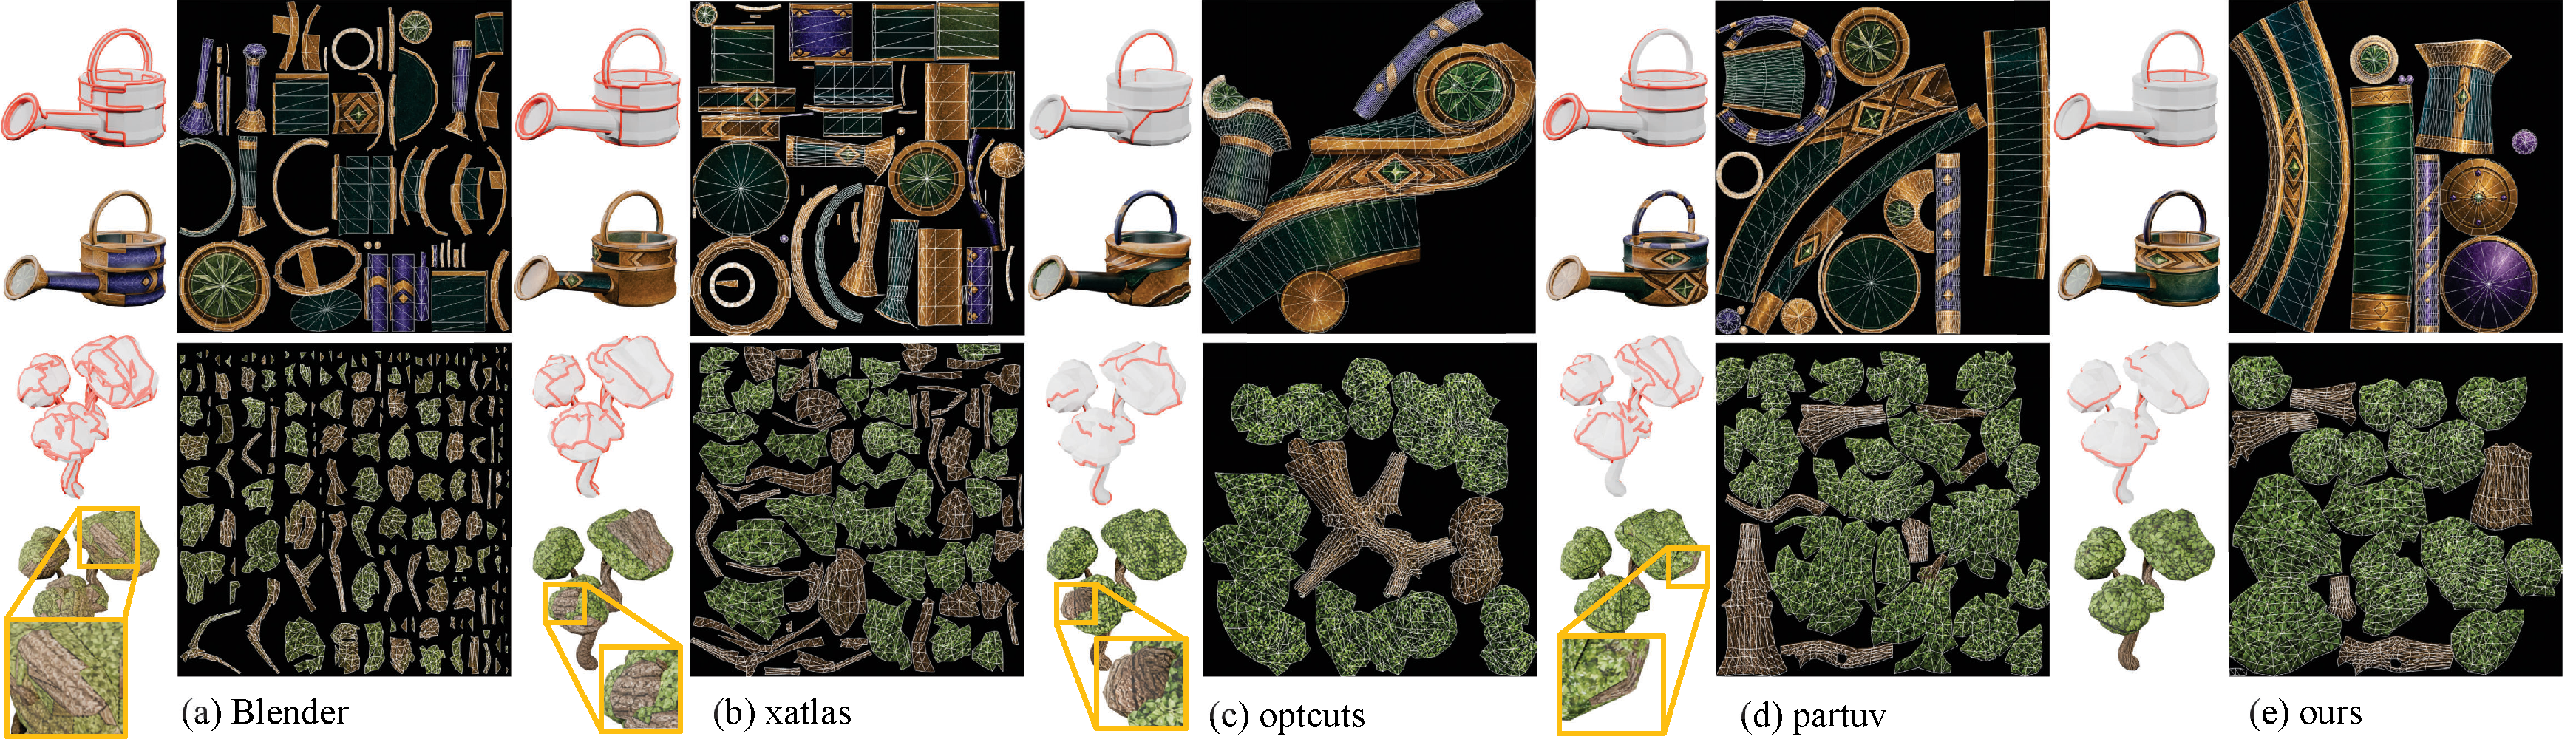
\includegraphics[width=\linewidth]{figures/comparison.pdf} 
    \caption{\textbf{Comparison.} We compare our \methodname{} against Blender's Smart UV Project~\cite{blender}, xatlas~\cite{young2019xatlas}, OptCuts~\cite{li2018optcuts}, and PartUV~\cite{wang2025partuv}.
    For each case, we show renderings with seams overlaid (upper left), the results of semantic-aware UV space texture generation (bottom left), and the corresponding UV space textures (right). Problematic regions are highlighted with yellow zoom-in boxes.
    } 
    \label{fig:comp_tex}
    \vspace{-4mm}
\end{figure*}

By alternating global context aggregation and local topology-aware update, the backbone captures both the global organization of seam layouts and the local evidence that determines where seams should lie. Since mesh edges are undirected, we process each edge in both directions during message passing and average the two directional edge features before prediction. The final edge features are normalized and projected to a scalar output for each mesh edge, yielding the edge-wise velocity field used in our flow matching model.

% Realizing the formulation above requires a neural architecture that parameterizes the velocity field directly on the mesh graph. Since the target seam layout is defined over mesh connectivity, a mesh-native graph network is a natural choice for this task. In particular, information propagation on the mesh graph provides an effective way to encode the local geometric structure that strongly influences seam placement.

% However, conventional graph neural networks (GNNs) are inherently local, with each layer propagating information only within a limited neighborhood, and capturing long range dependencies requires stacking many layers. This is problematic for seam generation: i) whether an edge should be selected as a seam often depends on its immediate geometric context, such as dihedral angle, local curvature, and proximity to sharp creases or part boundaries. ii) high quality seam layouts require global coordination across the entire surface, so that individual edge decisions collectively form connected, topologically valid cuts and partition the mesh into well shaped UV islands. Local information propagation alone is therefore insufficient to model the full seam layout distribution.

% To address this, we design a Mesh Transformer that combines local geometric aggregation with global context modeling (see the center of Fig.~\ref{fig:pipeline}). In each block, we first apply a global self-attention module over all vertices, allowing distant regions on the mesh to exchange information directly and enabling long-range coordination of seam decisions. We then apply a local message-passing module that updates vertex and edge features along mesh connectivity, refining predictions using local geometric structure in a topology-aware manner. By alternating these two modules throughout the network, our backbone captures both the local evidence and the global structural dependencies underlying artist-authored seam layouts, leading to seam predictions that are both geometrically precise and globally coherent.



\subsection{Conditional Seam Inpainting}
\label{sec:inpainting}
In production UV workflows, artists often refine an initial unwrap under partial constraints, such as protecting salient regions, enforcing selected seams, or revising charts that cause overlaps. 
We support this process with conditional seam inpainting, which reuses the learned flow model as a generative prior. 


Following conditional diffusion sampling~\cite{lugmayr2022repaint}, we clamp the known edges throughout the sampling process and let the model predict the unknown ones.
Let $\mathcal{K} \subset \mathcal{E}$ denote the set of known edges with target seam labels $e_1^{\mathcal{K}} \in \{0,1\}^{|\mathcal{K}|}$.
During sampling, we follow the same procedure as in unconditional generation, but overwrite the values of known edges at each step using their corresponding flow interpolation:
\[
e_{t,i} = t\, e_{1,i}^{\mathcal{K}} + (1-t)\, e_{0,i}, \quad i \in \mathcal{K},
\]
where $e_0$ is the initial Gaussian noise.
The updated $e_t$ is then passed to the Mesh Transformer for the next denoising step.
Because our backbone propagates information through both global self-attention and local message passing, the clamped edges serve as contextual constraints for the remaining editable edges, enabling coherent conditional seam generation.


This conditional inpainting mechanism enables two practical applications.
First, it supports constraint-guided seam completion.
Given sparse user-provided constraints, such as seam-free regions or edges that should be cut, \methodname{} resamples the unconstrained edges conditioned on these inputs.
The generated layout respects the prescribed constraints while remaining consistent with the learned artist-authored seam prior.
This provides a convenient form of coarse controllability: users specify high-level editing intent, and the model completes the remaining seam layout through conditional sampling.
Second, the same mechanism enables automatic localized self-refinement.
Since overlap-freeness is not explicitly enforced by the generative objective, a small number of sampled layouts may produce self-overlapping UV islands after parameterization.
For these cases, we keep the reliable parts of the seam layout fixed and treat only the region around the problematic island as editable.
Conditional inpainting then locally resamples seams in the affected region while preserving the rest of the layout.
This reuses the pretrained model as a local seam prior without requiring a separate repair network, additional training, or a handcrafted post-processing objective.

% In practical manual UV editing, artists interactively refine seams under partial constraints: certain visible or semantically important regions should remain seam-free, while some selected edges may be required as cuts to separate parts or resolve local parameterization issues. Since seam placement is inherently ambiguous and highly dependent on global shape context, completing the remaining layout from such partial constraints is difficult to achieve with handcrafted local rules. This motivates reusing the learned seam distribution as a conditional prior for interactive local seam editing.

% % Beyond unconditional seam generation, our trained flow model naturally supports training-free conditional seam inpainting. 
% Since seam layouts are represented as edge-wise variables on the mesh graph, any subset of edges can be treated as known conditions, while the remaining edges are regenerated by the same pretrained model. This allows \methodname{} to perform localized seam editing without training an additional model or optimizing a separate objective.

% Following the idea of conditional diffusion sampling~\cite{lugmayr2022repaint}, we clamp the known edges throughout the sampling process and let the model predict the unknown ones. Let $\mathcal{K} \subset \mathcal{E}$ denote the set of known edges with target seam labels $e_1^{\mathcal{K}} \in \{0,1\}^{|\mathcal{K}|}$. During sampling, we follow the same procedure as in unconditional generation, but overwrite the values of known edges at each step using their corresponding flow interpolation:
% \[
% e_{t,i} = t\, e_{1,i}^{\mathcal{K}} + (1-t)\, e_{0,i}, \quad i \in \mathcal{K},
% \]
% where $e_0$ is the initial Gaussian noise. The updated $e_t$ is then passed to the Mesh Transformer for the next denoising step. Since our backbone propagates information through both global self-attention and local message passing, the clamped edges provide contextual constraints for the remaining edges, enabling coherent local seam regeneration.

% This conditional inpainting mechanism enables two practical uses: constraint-guided seam generation and automatic self-refinement.
% First, it enables constraint guided local seam editing. Given user-provided sparse constraints, such as seam-free regions or edges to be cut, \methodname{} resamples the remaining unconstrained edges conditioned on these inputs, producing a seam layout that respects user intent while remaining consistent with the learned artist-authored distribution. This provides a convenient form of coarse local control, where users specify high-level constraints, and the model completes the layout through conditional sampling.
% %
% Second, the same mechanism can be used for automatic self-refinement. Since overlap-freeness is not explicitly enforced by the generative objective, a small number of sampled layouts may produce self-overlapping UV islands after parameterization. For these cases, we keep the reliable parts of the layout fixed and resample only a local region around the problematic island using conditional inpainting. This reuses the trained model as a local seam prior without requiring a separate repair model or additional training.
 

% Overall, post-sampling refinement does not require any extra training or separate optimization objective. It reuses the same generative model as a conditional seam prior, making \methodname{} applicable not only for fully automatic seam generation but also for interactive and localized UV layout correction.

% \subsection{Post-Sampling Refinement}
% \label{sec:refinement}
% After training, our model has learned to fit the distribution of artist-authored seam layouts, allowing it to generate seams that are globally plausible and consistent with artist-authored priors. However, since overlap-freeness is not explicitly enforced by the generative objective, distributional plausibility does not guarantee that every sampled seam layout can be flattened without error. This occasionally produces self-overlapping UV islands after parameterization.

% We address these failure cases through localized refinement. Rather than discarding the sample or introducing a separate repair model, we directly reuse the trained flow matching model for conditional seam inpainting. Specifically, \methodname{} admits standard training-free conditional sampling~\cite{lugmayr2022repaint} by fixing any subset of edges and using the pretrained model to generate the remaining edges without additional training. 
% Concretely, let $\mathcal{K} \subset \mathcal{E}$ denote the subset of edges with known target labels $e_1^{\mathcal{K}} \in {0,1}^{|\mathcal{K}|}$.
% During sampling, we follow the same procedure as in the base model, but for edges in $\mathcal{K}$, we replace their current values with the linear interpolation between the target seam labels and the initial noise,
% \[
% e_{t,i} = t\, e_{1,i}^{\mathcal{K}} + (1-t)\, e_{0,i}, \quad i \in \mathcal{K},
% \]
% and then feed the updated $e_t$ into the model for the next step. Since the Mesh Transformer propagates information through both global self-attention and local message passing, the clamped known edges condition the velocity predictions for the remaining edges throughout the denoising process.

 
% Based on the conditional inpainting mechanism which naturally supports localized UV correction and inspired by practical manual UV editing, 
% % when artists encounter an overlapping island, they may either insert additional seams inside the island to further subdivide it, or locally adjust the partition between the island and its neighboring regions. 
% we consider two refinement modes as shown in the Fig~\ref{fig:refine}. 

% % The first keeps the island boundary fixed and only re-generates seams in the interior, corresponding to local subdivision within the problematic island. 

% The first mode keeps the island boundary fixed and only re-generates seams in the interior, corresponding to local subdivision within the problematic island. Let $I$ be an overlapping island and let $\mathcal{E}^{\mathrm{int}}(I) \subset \mathcal{E}$ denote the edges strictly interior to $I$, i.e., edges whose endpoints both lie away from the UV boundary of $I$. We define the known subset as
% \[
% \mathcal{K}_{\mathrm{int}} = \mathcal{E} \setminus \mathcal{E}^{\mathrm{int}}(I),
% \]
% clamp $\mathcal{K}_{\mathrm{int}}$ to the current seam labels, and re-inpaint only $\mathcal{E}^{\mathrm{int}}(I)$. Because the boundary of $I$ is preserved, the rest of the atlas remains unchanged, and any newly introduced cuts can only appear inside $I$, subdividing it into smaller sub-islands. This mode is effective when the overlap is caused by insufficient internal seams.

% When modifying the island interior alone is not sufficient, we switch to the second mode.
% % and enlarge the resampled region around the problematic island. 
% The second allows a larger local neighborhood around the island boundary to be re-generated, so that the island can be repartitioned together with its immediate neighbors while the rest of the atlas remains fixed.
% Let $\mathcal{N}(I)$ denote the set of UV islands that share at least one boundary edge with $I$, and let $\mathcal{E}^{\mathrm{bd}}(I)$ denote the boundary edges of $I$. We define the resampled region as
% \[
% \mathcal{U}_{\mathrm{bd}} = \mathcal{E}^{\mathrm{bd}}(I) \;\cup\; \bigcup_{J \in \mathcal{N}(I)} \mathcal{E}^{\mathrm{int}}(J),
% \]
% and use
% \[
% \mathcal{K}_{\mathrm{bd}} = \mathcal{E} \setminus \mathcal{U}_{\mathrm{bd}}
% \]
% as the known subset. Clamping $\mathcal{K}_{\mathrm{bd}}$ and re-inpainting $\mathcal{U}_{\mathrm{bd}}$ allows the problematic island to grow or shrink against its immediate neighbors, while keeping regions beyond the 1-hop neighborhood fixed. This provides greater flexibility when the overlap is rooted in an unsuitable local boundary partition rather than a lack of internal seams.

% \begin{figure}[t]
%     \centering
%     \includegraphics[width=\linewidth]{figures/inpainting.pdf}
%     \caption{\textbf{Two modes of \methodname{} refinement.}}
%     \label{fig:refine}
% \end{figure}

